\subsubsection{Synthesis of Nanomolecular Metal-Oxo Clusters with Manifold Applications}
\index{Kortz, Ulrich}

\paragraph{Research Team}
Ulrich Kortz (Professor), Bernd von der Kammer (Research Assistant), Santiago Reinoso
(Postdoctoral Fellow), Elena Chubarova (Postdoctoral Fellow), Michael Dickman (Senior
Research Associate), Firasat Hussain (PhD Student), Bassem Bassil (PhD Student), Sib
Sankar Mal (PhD Student), Nadeen Nsouli (PhD Student), Luis Piedra-Garza (PhD Student),
Amal Ismail (PhD Student),
Isabella Roemer (MS Student) \ \ \\ \ \ \\

%%% give a very short (150 words description of your research area)

The general research activity of the Kortz group at
IUB is in the field of synthetic inorganic and organometallic
chemistry. We are particularly interested in the preparation and
structural characterization of large molecular assemblies called
polyoxometalates. Polyoxometalates (or polyoxoanions) are
metal-oxygen clusters with a tremendous structural variety and
interesting properties in different fields including catalysis,
medicine and materials science. The multitude of potential
applications has led to significant interest in polyoxometalates
worldwide. Our research activities are mainly focused on (a)
hybrid organic-inorganic polyoxoanions and (b) transition
metal-substituted polyoxoanions. The former class is of potential
interest in medicine (virus and tumor inhibition, e.g. AIDS) and
the latter in the areas of chemical and electrochemical catalysis
(e.g. oxidation of organic substrates by dioxygen) and materials
science (e.g. sensor technology, single-molecule magnets).
Polyoxoanions are synthesized and structurally characterized at
IUB using a multitude of solution and solid-state analytical
techniques (e.g. NMR, XRD, IR, UV-Vis, AA). Investigation of the
properties of our novel compounds is also accomplished in
collaboration with expert colleagues from around the world (e.g.
Prof. N. Dalal, Florida State University, USA and Prof. L. Nadjo,
Universit\'{e} Paris-Sud, France).



\paragraph{Highlights}

%%% give a short (500 words)description of the research highlights. 1 figure costs 100 words

{\sl Supramolecular Chemistry}: Wheel-Shaped Poly\-oxo\-tungstate
\BPChem{[Cu\_{20}Cl(OH)\_{24}(H\_{2}O)\_{12}(P\_{8}W\_{48}O\_{184})]\^{25-}} Macro\-anion
Forms Supramolecular "Blackberry" Structure in Aqueous Solution\\
\\
The hydrophilic polyoxotungstate
\BPChem{[Cu\_{20}Cl(OH)\_{24}(H\_{2}O)\_{12}(P\_{8}W\_{48}O\_{184})]\^{25-}}
$(\mathbf{Cu}_{20}\mathbf{P}_8\mathbf{W}_{48})$ self-assembles into single-layer, hollow,
spherical "blackberry"-type structures in aqueous solutions, as studied by DLS, SLS, zeta
potential analysis and SEM techniques (Fig.~\ref{kortzfig1}). This represents the first
report of blackberry formation for a non-Mo-containing polyoxometalate. The shape and size
of the blackberries do not change during the slow blackberry formation process, neither
with polyanion concentration nor with temperature. Our results suggest that blackberry
formation is most likely a general phenomenon for hydrophilic polyanions with suitable
size and charge in a polar solvent, and not a specific property of polyoxomolybdates and
their derivatives. The $\mathbf{Cu}_{20}\mathbf{P}_8\mathbf{W}_{48}$ polyanions are so far
the smallest type of polyanions (equivalent radius \mbox{$<2\;nm$}) to date showing the
unique self-assembly behavior, helping us to move one step closer towards identifying the
transition point from simple ions (can be described by the Debye-H\"{u}ckel theory) to
polyanions in very dilute solutions.



% to include a figure, generate a file xxx.pdf and integrate the following lines
\begin{figure}[ht]
  \begin{center}
    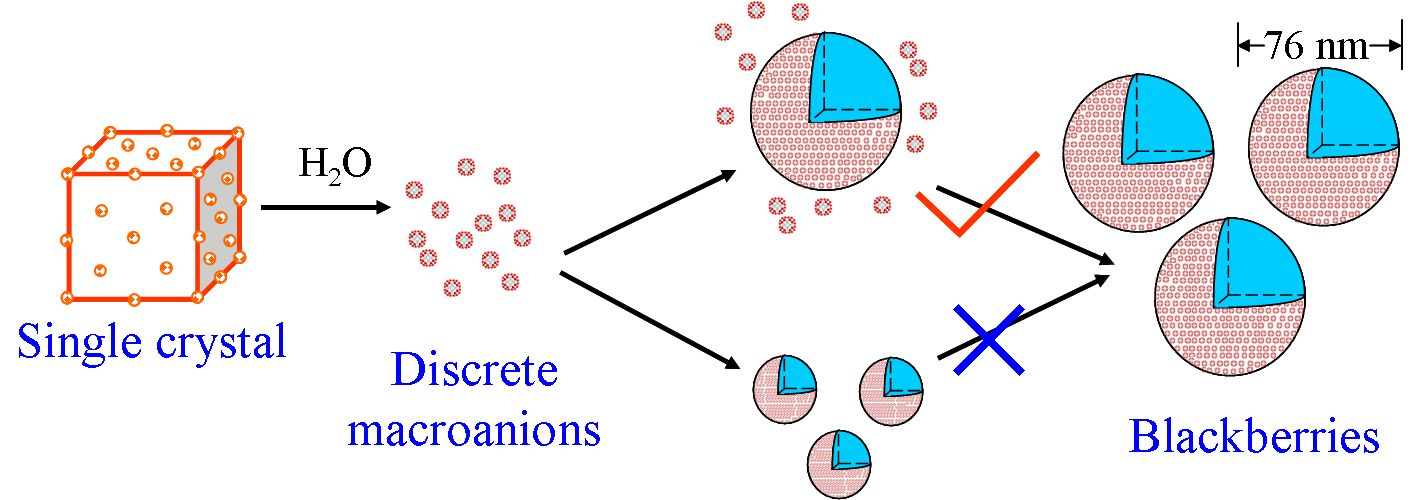
\includegraphics[width=7cm]{Kortz/kortzfig1}
    \mycaption{Possible mechanisms of $\mathbf{Cu}_{20}\mathbf{P}_8\mathbf{W}_{48}$
      blackberry formation in dilute aqueous solution. On the basis of SLS and DLS
      results, the upper mechanism has been proven to be correct, while the bottom
      mechanism can be ruled out.}\label{kortzfig1}
  \end{center}
\end{figure}
% to reference it use ``Figure.~\ref{fig:xxx}''; the numbers will be computed automatically.

{\sl Molecular Magnetism}: Observation of a Half Step Magnetization
in the \BPChem{\{Cu\_3\}}-Type Triangular Spin Ring\\
\\
We report pulsed field magnetization and ESR experiments on a \BPChem{\{{Cu\_3}\}}
nanomagnet, where antiferromagnetically coupled \BPChem{Cu\^{2+}} ($S = \frac{1}{2}$) ions
form a slightly distorted triangle. The remarkable feature is the observation of a half
step magnetization, hysteresis loops, and an asymmetric magnetization between a positive
and a negative field in a fast sweeping external field (Fig.~\ref{kortzfig2}). This is
attributed to an adiabatic change of magnetization. The energy levels determined by ESR
unveil that the different mixing nature of a spin chirality of a total $S = \frac{1}{2}$
Kramers doublet by virtue of Dzyaloshinskii-Moriya interactions is decisive for inducing
half step magnetization.

\begin{figure}[ht]
\begin{center}
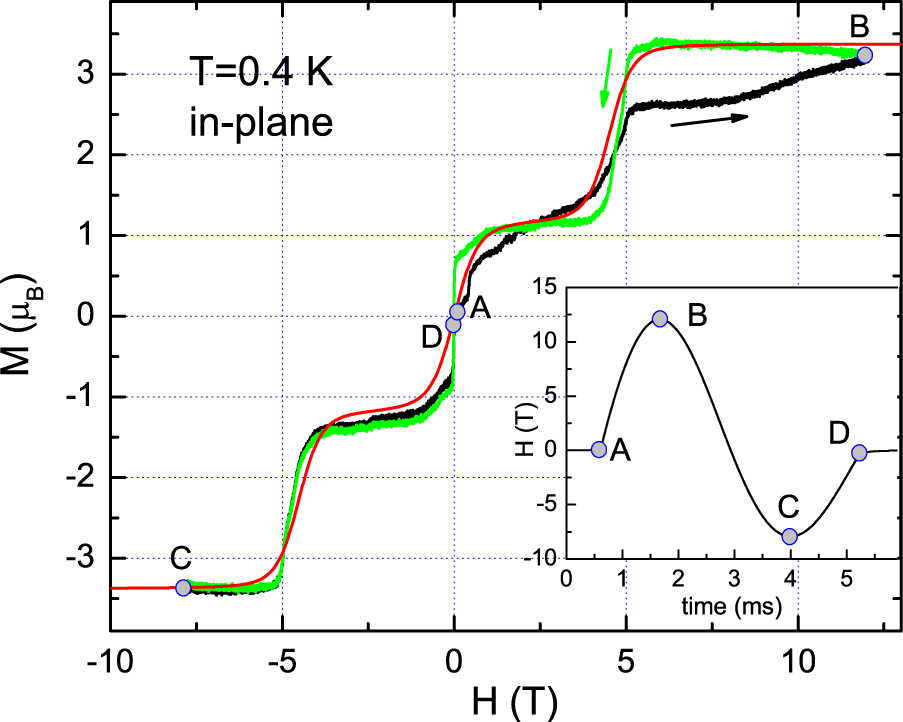
\includegraphics[width=7cm]{Kortz/kortzfig2}
\caption{Magnetization curve vs pulsed magnetic field at 0.4 K.  The saturated
  magnetization is scaled to $g \mu_BS$. The thin line is the calculated isothermal
  magnetization curve. Arrows denote sweep directions $(A \rightarrow B \rightarrow C
  \rightarrow D)$. The inset shows the pulsed magnetic field versus time.}
\label{kortzfig2}
\end{center}
\end{figure}


{\sl Oxidation Catalysis}: Bio-Inspired Oxidations with
Polyoxometalate Catalysts\\
\\
Transition metal-substituted polyoxometalates (TMSP) provide a redox-active metal center
(e.g. Mn, Fe, Ru) with a totally inorganic ligand system, featuring rigid polydentate
binding sites, high electron-acceptor character, extreme robustness and interesting
structural and coordination properties, in some cases, mimicking the coordination geometry
of natural oxygenase enzymes.  The synthesis and reactivity of TMSPs can be promoted by
microwave (MW) induced dielectric heating. Iron(III)-containing POMs with nuclearities
1-4, namely \BPChem{[$\alpha$-Fe(H\_2O)SiW\_{11}O\_{39}]\^{5-}},
\BPChem{[$\gamma$-Fe\_2(H\_2O)\_2SiW\_{10}O\_{38}]\^{6-}},
\BPChem{[$\alpha$-Fe\_3(H\_2O)\_3SiW\_9 O\_{37}]\^{7-}} and
\BPChem{[$\beta$-Fe\_4(H\_2O)\_{10}(XW\_9O\_{33})\_2]\^{n-}} (\BPChem{X = Se\^{IV},
  Te\^{IV}; As\^{III}, Sb\^{III}}; n $= 4,6$) were found to catalyze the MW assisted
cyclohexane oxygenation with high turnover frequencies. Preliminary results indicate that
the Krebs-type Fe-polyoxotungstates can also promote the oxidative cleavage of
3,5-ditert-butylcatechol with molecular oxygen.\\
\\
{\sl Nanomolecular Science}: STM/STS Observation of Polyoxoanions
on HOPG Surfaces\\
\\
A combination of scanning tunneling microscopy (STM) and scanning tunneling spectroscopy
(STS) techniques have been performed on the wheel-shaped
\BPChem{[Cu\_{20} Cl(OH)\_{24} (H\_2O)\_{12} (P\_8 W\_{48} O\_{184})]\^{25-}} and the
ball-shaped
\BPChem{[\{Sn(CH\_3)\_2 (H\_2O)\}\_{24} \{Sn(CH\_3)\_2\}\_{12}
  ($A$-PW\_9 O\_{34})\_{12}]\^{36-}}
deposited on highly oriented pyrolytic graphite (HOPG) surfaces.  Small, regular molecule
clusters as well as separated single molecules were observed. The size of the molecules is
in agreement with the data determined by X-ray crystallography. In STS measurements, we
found a rather large contrast at the expected location of the Cu metal centers in our
molecules, i.e. the location of the individual Cu ions in their organic matrix is directly
addressable by STS.


\paragraph{Collaborations}
\begin{enumerate}
\item {\sl International University Bremen}\\ Prof. Ryan Richards\\
  Preparation of Heterogeneous Catalytic Systems\\
  Prof. Werner Nau\\
  Structural Characterization of Host-Guest Complexes
\item{\sl Universit\"at Erlangen-N\"urnberg} \\ Prof. Paul M\"uller \\
  Surface Science of Polyoxometalates using STM and STS
\item {\sl Universit\"at Osnabr\"uck}\\ Prof. Manfred Neumann\\
  XPS and Magnetic Studies of Polyoxometalates\\
  Prof. J\"urgen Schnack \\ Numerical Diagonalization of Spin
  Hamiltonians\\
  Prof. Andrei V. Postnikov\\
  Density Functional Calculations
\item {\sl Florida State University, USA} \\ Prof. Naresh S. Dalal \\Magnetism and EPR of
  Polyoxometalates
  \\Prof. Alan G. Marshall\\
  High Resolution Mass Spectrometry of Polyoxometalates
\item {\sl Universit\'{e} Paris-Sud, France} \\ Prof. Louis Nadjo\\
  Electrochemistry and Electrocatalysis of Polyoxometalates
\item {\sl Universit\'{a} di Padova, Italy}\\ Prof. Marcella Bonchio\\Microwave-Assisted
  Oxidation Catalysis by Polyoxometalates
\item {\sl Universidad de Valencia, Spain} \\ Prof. Eugenio Coronado \\ Magnetic Studies
  of Polyoxometalates
\item {\sl Universitat Rovira i Virgili, Tarragona, Spain}\\
  Prof. Josep M. Poblet\\
  Computational Studies on Polyoxometalates
\item {\sl Catalysis Research Center, Sapporo, Japan}\\
  Prof. Masahiro Sadakane\\
  Structural Characterization of Ruthenium-Containing Polyoxometales
\item {\sl Tohuko University, Sendai, Japan} \\ Prof. Hiroyuki Nojiri\\
  High Field Magnetization of Polyoxometalates
\end{enumerate}

\paragraph{Grants}
% list the running grants in 2005, if none have been received, please delete this
% subsection.
\begin{enumerate}
\item Funded by DFG, \emph{Molecular Magnetism} \\

\item {\sl DFG}, (priority program 1118, Secondary Interactions as a Steering
  Principle for the Selective Functionalization of Non-Reactive Substrates),
  Ph.D. Fellowship for Nadeen Nsouli \item {\sl EU-COST D29}, Novel Sustainable Metal
  Catalyzed Oxidations with \BPChem{H\_2O\_2} and \BPChem{O\_2}
\item Chemical Industry (confidential), Postdoctoral Fellowship for Dr. Elena
  Chubarova \item {\sl Basque Government}, Postdoctoral Fellowship for Dr. Santiago
  Reinoso \item Graduiertenkolleg 1213, Ph.D. Fellowship for Luis Piedra-Garza
\item Egyptian Government, Ph.D. Fellowship for Amal Ismail
\end{enumerate}

\paragraph{Awards, Prizes}
\begin{enumerate}
\item Initiator and coordinator of agreement between the School of Engineering and
  Science, International University Bremen and the Catalysis Research Center, Hokkaido
  University, in order to further strengthen the mutual relationship and to encourage
  scientific exchange.
\item Editorial Board Member, \emph{Journal of Cluster Science}, Springer
\item Invited as external expert for EU-COST D26/0015 (Understanding and predicting the
  electronic, magnetic and structural properties of polyoxometalates) Working Group
  Meeting at Strasbourg University, 29-30 September 2006, Seminar Title ''Synthetic
  Strategies Towards Polyoxometalates with Novel Shapes, Sizes, Compositions and
  Functions''
\item Several Invited Lectures (Rome, Giessen, Dnepropetrovsk, Washington DC, Houston,
  Rostock)
\end{enumerate}

\paragraph{Patents}
\begin{enumerate}
\item Supported polyoxometalates and process for their preparation (Kortz, U.; Bi, L.-H.;
  Richards, R.; Zhu, K.)
\item Novel Ru-substituted polyoxometalates and process for their preparation (Kortz, U.;
  Bi, L.-H.)
\item Novel Pd- and Pt-substituted polyoxometalates and process for their preparation
  (Kortz, U.; Bi, L.-H.)
\item Novel transition metal substituted polyoxometalates and process for their
  preparation (Kortz, U.; Hussain, F.; Mal, S. S.)
\item Process for producing phenols (Kortz, U.; Bi, L.-H.; Chubarova, E.)
\end{enumerate}

\paragraph{Activities (IUB)}
\begin{enumerate}
\item  Member, Nanomolecular Science Recruitment Committee
\item Member, Nanomolecular Science Curriculum Committee
\item Member, Research Development Committee
\item Member, Committee on Administrative Support and Infrastructure
\item Member, Academic Integrity Committee
\item Organizer, Wednesday Colloquium
\item Seminar, University Club Lecture Series
\end{enumerate}


\nocite{Kortz1}
\nocite{Kortz2}
\nocite{Kortz3}
\nocite{Kortz4}
\nocite{Kortz5}
\nocite{Kortz6}
\nocite{Kortz7}
\nocite{Kortz8}
\nocite{Kortz9}
\nocite{Kortz10}
\nocite{Kortz11}
\nocite{Kortz12}
\nocite{Kortz13}
\nocite{Kortz14}
\nocite{Kortz15}
\nocite{Kortz16}
\nocite{Kortz17}
\nocite{Kortz18}
\nocite{Kortz19}



%\paragraph{Publications}
%\nocite{uk01} \nocite{uk02} \nocite{uk03} \nocite{uk04}
%\nocite{uk05} \nocite{uk06} \nocite{uk07} \nocite{uk08}
%\nocite{uk09} \nocite{uk10} \nocite{uk11} \nocite{uk12}
%\nocite{uk13} \nocite{uk14} \nocite{uk15} \nocite{uk16}
%\nocite{uk17} \nocite{uk18}



%\begin{description}
%  \item[Journals] Inorg. Chem.~\cite{uk01},
%    J. Appl. Phys.~\cite{uk02}, Inorg. Chem.~\cite{uk03},
%    Inorg. Chem.~\cite{uk04}, Inorg. Chem.~\cite{uk05},
%    Adv. Synth. Cat.~\cite{uk06}, Chem. Commun.~\cite{uk07},
%    Electrochem. Comm.~\cite{uk08}, Eur. J. Inorg. Chem.~\cite{uk09},
%    Angew. Chem. Int. Ed.~\cite{uk10},
%    Angew. Chem. Int. Ed.~\cite{uk11}, Polyhedron~\cite{uk12},
%    Inorg. Chem.~\cite{uk13}, Chem. Commun.~\cite{uk14},
%    Inorg. Chem.~\cite{uk15}, J. Clust. Sci.~\cite{uk16}, Comptes
%    Rendus Chimie~\cite{uk17}, J. Mol. Cat. A~\cite{uk18}
%  \item[Conference Proceedings] CADE~\cite{Kohlhase:CADE1}, ...
%  \item[Books/Collections] \ldots
%\end{description}

%\cleardoublepage
%\bibliography{ses}
%\bibliographystyle{unsrt}

%%% Local Variables:
%%% mode: latex
%%% TeX-master: "RP-EECS"
%%% End:
